\section{习题一 \ 最佳平方逼近多项式}
下面即为绘制代码。
\inputpython{E:/numerical-approximation/code/p4/first/one.py}{1}{56}


\begin{figure}[htbp]
    \centering
    \subfigure[$k=1$]
    {
        \begin{minipage}[b]{.4\linewidth}
            \centering
            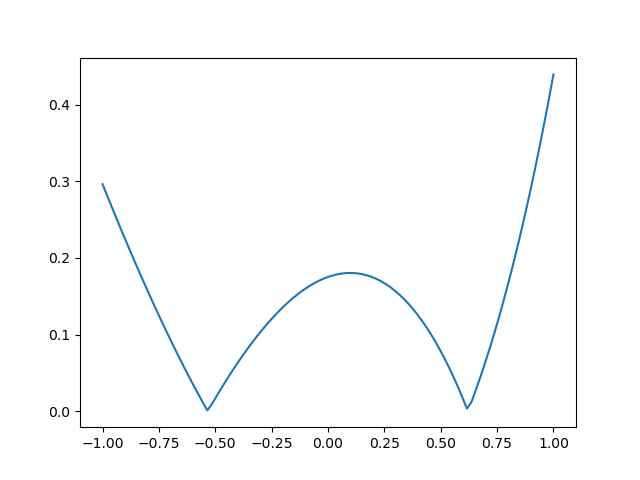
\includegraphics[scale=0.29]{pic/1/exk=1.png}
        \end{minipage}
    }
    \subfigure[$k=3$]
    {
        \begin{minipage}[b]{.4\linewidth}
            \centering
            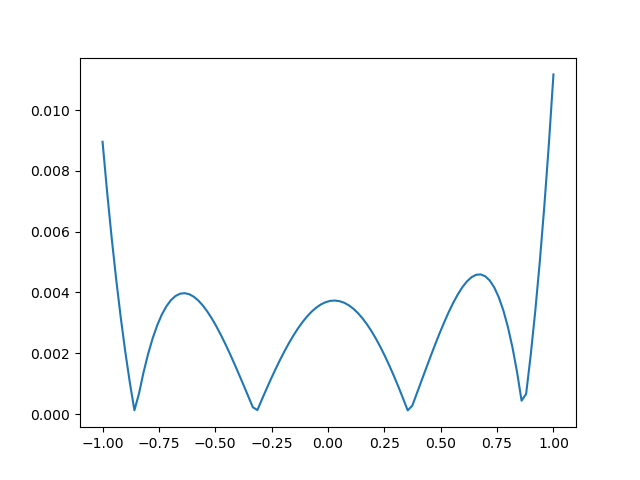
\includegraphics[scale=0.29]{pic/1/exk=3.png}
        \end{minipage}
    }
    \subfigure[$k=5$]
    {
        \begin{minipage}[b]{.4\linewidth}
            \centering
            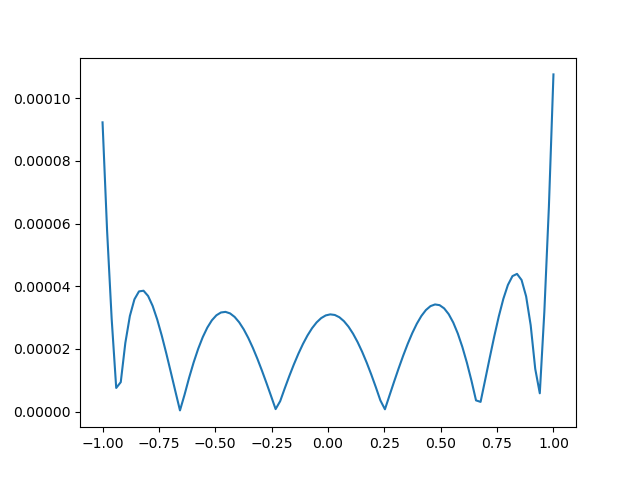
\includegraphics[scale=0.29]{pic/1/exk=5.png}
        \end{minipage}
    }
    \subfigure[$k=10$]
    {
        \begin{minipage}[b]{.4\linewidth}
            \centering
            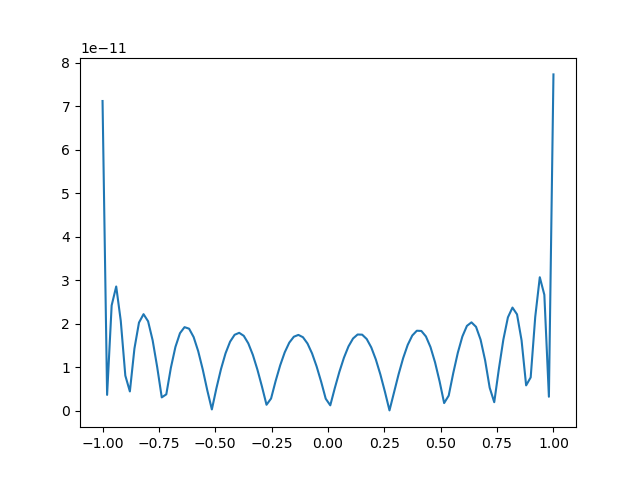
\includegraphics[scale=0.29]{pic/1/exk=10.png}
        \end{minipage}
    }
    \caption{$e^x$最佳平方逼近多项式}
\end{figure}

\begin{figure}[h]
    \centering
    \subfigure[$k=1$]
    {
        \begin{minipage}[b]{.4\linewidth}
            \centering
            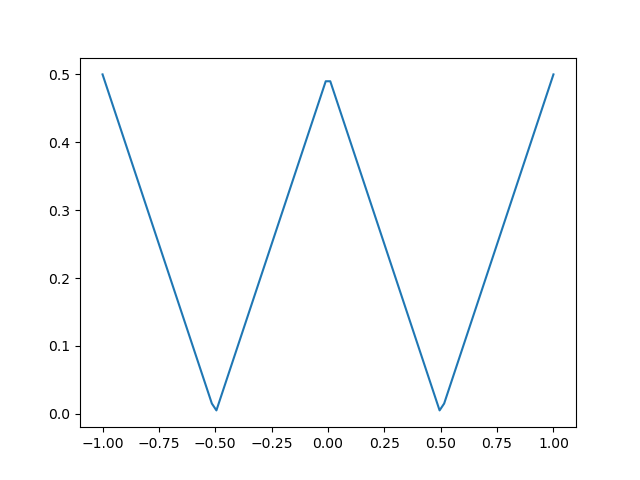
\includegraphics[scale=0.29]{pic/1/absk=1.png}
        \end{minipage}
    }
    \subfigure[$k=3$]
    {
        \begin{minipage}[b]{.4\linewidth}
            \centering
            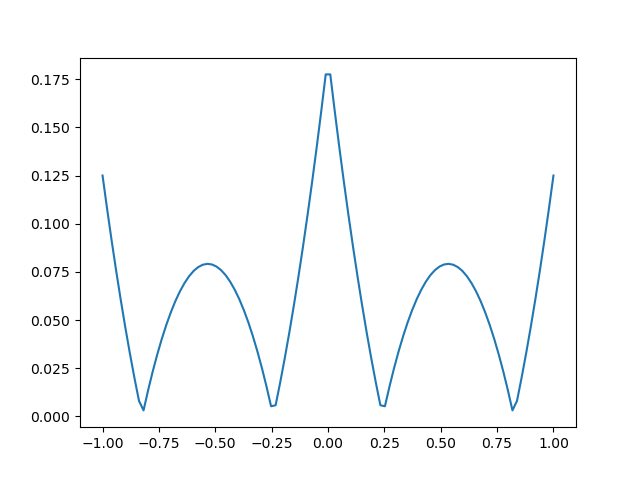
\includegraphics[scale=0.29]{pic/1/absk=3.png}
        \end{minipage}
    }
    \subfigure[$k=5$]
    {
        \begin{minipage}[b]{.4\linewidth}
            \centering
            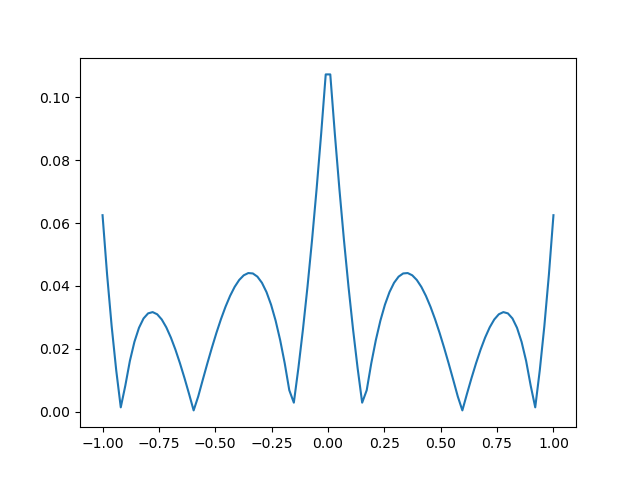
\includegraphics[scale=0.29]{pic/1/absk=5.png}
        \end{minipage}
    }
    \subfigure[$k=10$]
    {
        \begin{minipage}[b]{.4\linewidth}
            \centering
            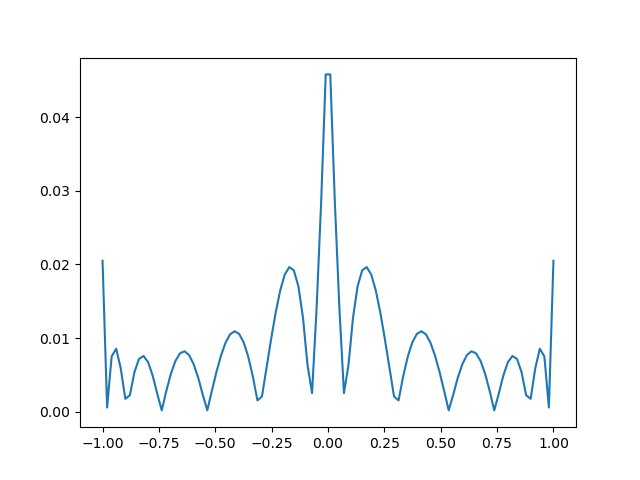
\includegraphics[scale=0.29]{pic/1/absk=10.png}
        \end{minipage}
    }
    \caption{$|x|$最佳平方逼近多项式}
\end{figure}

\vspace{10em}
以下为$\Delta_k \sim k$曲线绘制代码
\inputpython{E:/numerical-approximation/code/p4/first/1_2_3.py}{1}{20}

\begin{figure}[htbp]
    \centering

    {
        \begin{minipage}[b]{.9\linewidth}
            \centering
            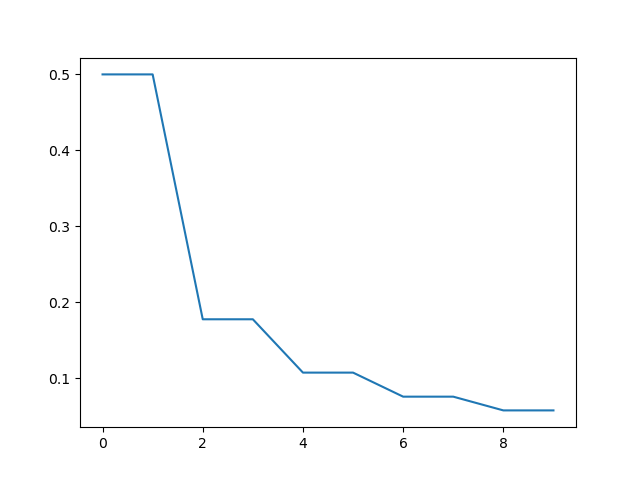
\includegraphics[scale=0.5]{pic/1/2_delta_k.png}
        \end{minipage}
    }


    \caption{$\Delta_k \sim k$}
    \centering

    {
        \begin{minipage}[b]{.9\linewidth}
            \centering
            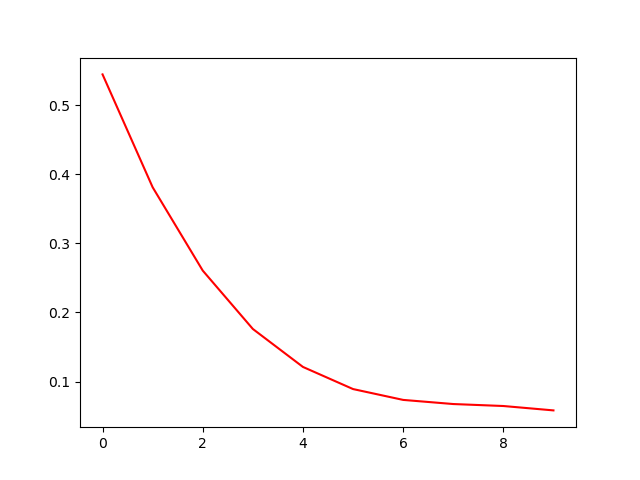
\includegraphics[scale=0.5]{pic/1/curve_fit.png}
        \end{minipage}
    }


    \caption{$\Delta_k \sim k$最小二乘拟合}
\end{figure}


\clearpage
\section{习题二 \ 正交多项式的应用}
注:由于代码过长,不在页面进行展示。
\begin{figure}[htbp]
    \centering

    {
        \begin{minipage}[b]{.9\linewidth}
            \centering
            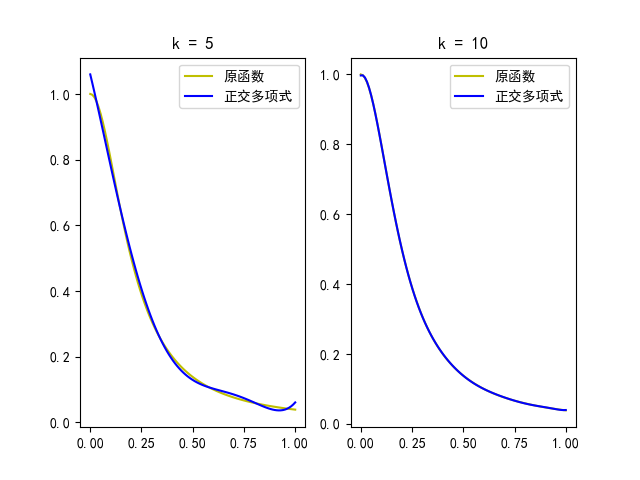
\includegraphics[scale=0.6]{pic/2/1.png}
        \end{minipage}
    }


    \caption{$\{x^i\}$为基函数}

\end{figure}

\begin{figure}[htbp]
    \centering

    \subfigure[$k=5$]
    {
        \begin{minipage}[b]{.9\linewidth}
            \centering
            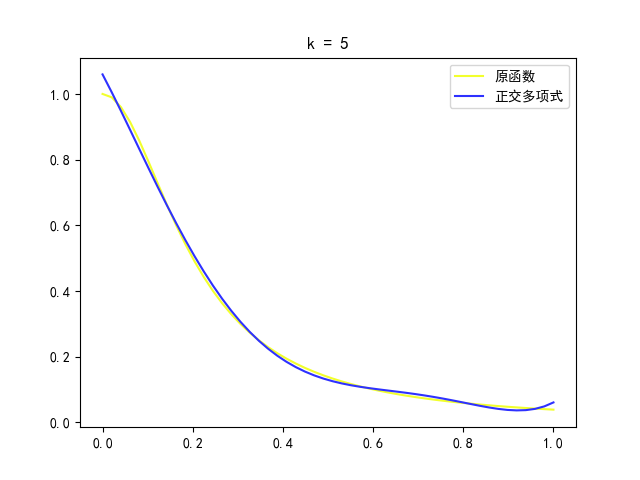
\includegraphics[scale=0.29]{pic/2/2k=5.png}
        \end{minipage}
    }
    \subfigure[$k=10$]
    {
        \begin{minipage}[b]{.9\linewidth}
            \centering
            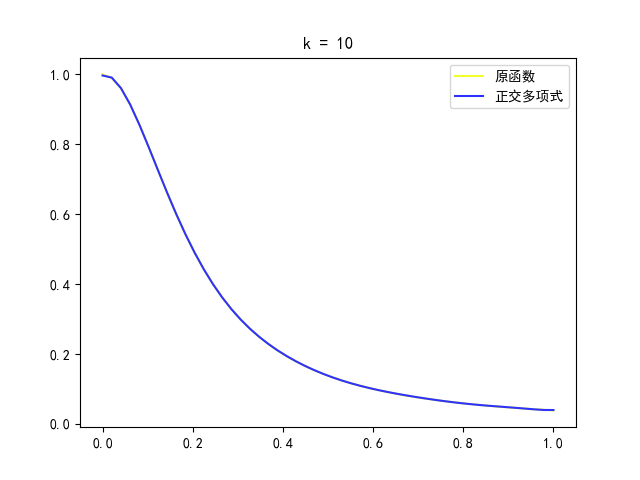
\includegraphics[scale=0.29]{pic/2/2k=10.png}
        \end{minipage}
    }

    \caption{$Legendre$多项式为基函数}
    \centering

    \subfigure[$k=5$]
    {
        \begin{minipage}[b]{.9\linewidth}
            \centering
            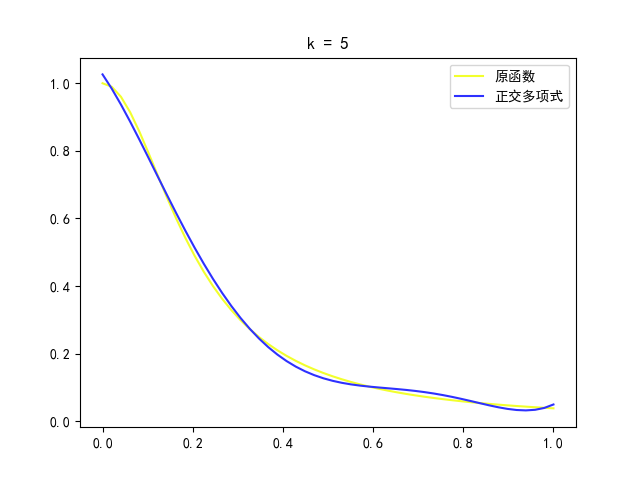
\includegraphics[scale=0.29]{pic/2/3k=5.png}
        \end{minipage}
    }
    \subfigure[$k=10$]
    {
        \begin{minipage}[b]{.9\linewidth}
            \centering
            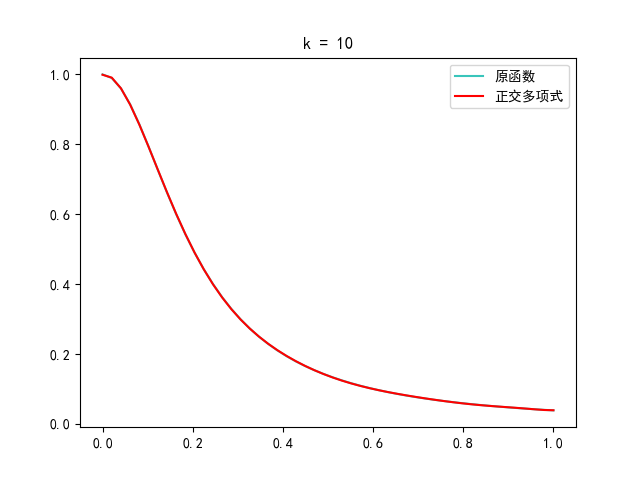
\includegraphics[scale=0.29]{pic/2/3k=10.png}
        \end{minipage}
    }

    \caption{$Chebyshev$多项式为基函数}
\end{figure}

\clearpage
\section{习题三 \ 多项式最小二乘法}
将三个问题的图像绘制在一起如下图:
\begin{figure}[htbp]
    \centering

    {
        \begin{minipage}[b]{.9\linewidth}
            \centering
            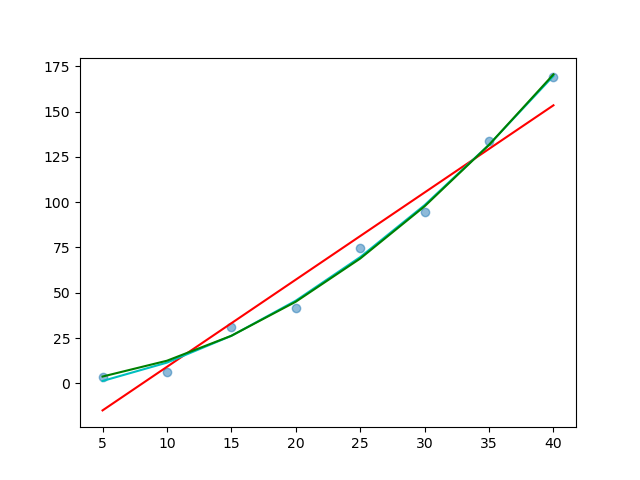
\includegraphics[scale=0.5]{pic/3/3.png}
        \end{minipage}
    }


    \caption{多项式最小二乘法}
    
\end{figure}

根据如上图像进行分析可知当$a_0 = 0, 即y = a_1x + a_2x^2$时拟合出来的更加合适。
\clearpage
\section{习题四 \ 指数函数最小二乘法}
画图对比如下:
\begin{figure}[htbp]
    \centering

    {
        \begin{minipage}[b]{.9\linewidth}
            \centering
            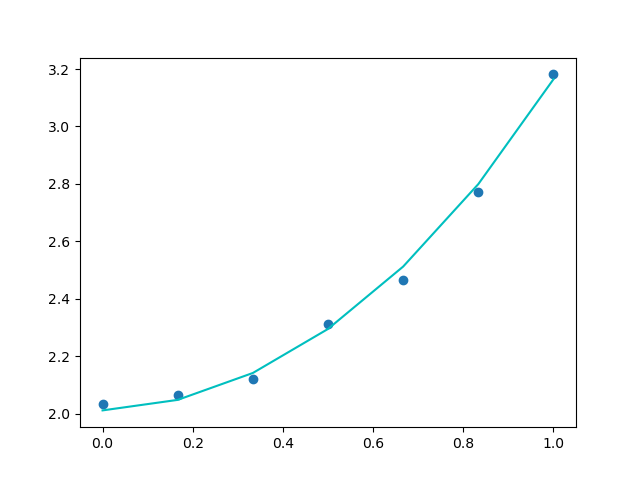
\includegraphics[scale=0.5]{pic/4/4.png}
        \end{minipage}
    }


    \caption{指数函数最小二乘法}
    
\end{figure}